%!TEX program = xelatex

\documentclass[11pt,titlepage]{report}
%!TEX root = main.tex

\usepackage[T1]{fontenc}
\usepackage{lmodern}
\usepackage[svgnames]{xcolor}
\usepackage{fontspec} % XeLaTeX required!
\usepackage{graphicx}
\usepackage{circuitikz}
\usepackage{tikz}
\usepackage{pifont}
\usepackage[some]{background}
\usepackage{xltxtra} 
\usepackage{setspace}
\usepackage[absolute]{textpos}
\usepackage[latin1]{inputenc}
\usepackage[english]{babel}
\usepackage{graphicx}
\usepackage{wrapfig}
\usepackage{fullpage}
\usepackage[margin=1in]{geometry}
\usepackage{float}
\usepackage{url}
\usepackage{multicol}
\usepackage{hyperref}
\usepackage{titlepic}
\usepackage{standalone}
\usepackage{siunitx}
\usepackage{booktabs}
\usepackage{amsmath}
\usepackage{unicode-math}
\usepackage{verbatim}
\usepackage{enumitem}
\usepackage{listings}
\usepackage{multirow}
\usepackage{pgfplots}
\pgfplotsset{compat=1.8}
\usepackage{caption} 
\usepackage[parfill]{parskip}
\usepackage{import}
\usepackage[backend=bibtexu,texencoding=utf8,bibencoding=utf8,style=ieee,sortlocale=en_GB,language=auto]{biblatex}
\usepackage[strict,autostyle]{csquotes}
\usepackage[final]{pdfpages}
\usepackage{subcaption}
\usepackage{ifplatform}
%\captionsetup[table]{skip=10pt}


% Fix for includepdf bug in Mac OS X
\newcommand{\insertpdfpath}[1]{
	\ifwindows
	\newcommand{\insertpdf}[2]{\includepdf[pages=##1]{##2}}
	\else
	\newcommand{\insertpdf}[2]{\includepdf[pages=##1]{#1/##2}}
	\fi
}

%set fonts
\setmainfont[Ligatures=TeX]{Myriad Pro}
\setmathfont{Asana Math}
\setmonofont{Lucida Console}

\usepackage{titlesec, color}
\renewcommand{\familydefault}{\sfdefault} %set font family
\renewcommand{\arraystretch}{1.2} %set table vertical spacing
\setlength\parindent{0pt} %no paragraph indent
\hypersetup{ %setup hyperlinks
    colorlinks,
    citecolor=black,
    filecolor=black,
    linkcolor=black,
    urlcolor=black
}

%redesign chapter headings
\definecolor{gray75}{gray}{0.75}
\newcommand{\chapternumber}{\thechapter}
\newcommand{\hsp}{\hspace{20pt}}
\titleformat{\chapter}[hang]{\Huge\bfseries}{\chapternumber\hsp\textcolor{gray75}{|}\hsp}{0pt}{\Huge\bfseries}

%Redefine appendix headers
\renewcommand{\appendixname}{Appendix}
\renewcommand{\appendixtocname}{Appendices}
\renewcommand{\appendixpagename}{Appendices}

%For code listings
\definecolor{black}{rgb}{0,0,0}
\definecolor{browntags}{rgb}{0.65,0.1,0.1}
\definecolor{bluestrings}{rgb}{0,0,1}
\definecolor{graycomments}{rgb}{0.4,0.4,0.4}
\definecolor{redkeywords}{rgb}{1,0,0}
\definecolor{bluekeywords}{rgb}{0.13,0.13,0.8}
\definecolor{greencomments}{rgb}{0,0.5,0}
\definecolor{redstrings}{rgb}{0.9,0,0}
\definecolor{purpleidentifiers}{rgb}{0.01,0,0.01}


\lstdefinestyle{csharp}{
language=[Sharp]C,
showspaces=false,
showtabs=false,
breaklines=true,
showstringspaces=false,
breakatwhitespace=true,
escapeinside={(*@}{@*)},
columns=fullflexible,
commentstyle=\color{greencomments},
keywordstyle=\color{bluekeywords}\bfseries,
stringstyle=\color{redstrings},
identifierstyle=\color{purpleidentifiers},
basicstyle=\ttfamily\small}

\lstdefinestyle{c}{
language=C,
showspaces=false,
showtabs=false,
breaklines=true,
showstringspaces=false,
breakatwhitespace=true,
escapeinside={(*@}{@*)},
columns=fullflexible,
commentstyle=\color{greencomments},
keywordstyle=\color{bluekeywords}\bfseries,
stringstyle=\color{redstrings},
identifierstyle=\color{purpleidentifiers},
}

\lstdefinestyle{matlab}{
language=Matlab,
showspaces=false,
showtabs=false,
breaklines=true,
showstringspaces=false,
breakatwhitespace=true,
escapeinside={(*@}{@*)},
columns=fullflexible,
commentstyle=\color{greencomments},
keywordstyle=\color{bluekeywords}\bfseries,
stringstyle=\color{redstrings},
identifierstyle=\color{purpleidentifiers}
}

\lstdefinestyle{vhdl}{
language=VHDL,
showspaces=false,
showtabs=false,
breaklines=true,
showstringspaces=false,
breakatwhitespace=true,
escapeinside={(*@}{@*)},
columns=fullflexible,
commentstyle=\color{greencomments},
keywordstyle=\color{bluekeywords}\bfseries,
stringstyle=\color{redstrings},
identifierstyle=\color{purpleidentifiers}
}

\lstdefinestyle{xaml}{
language=XML,
showspaces=false,
showtabs=false,
breaklines=true,
showstringspaces=false,
breakatwhitespace=true,
escapeinside={(*@}{@*)},
columns=fullflexible,
commentstyle=\color{greencomments},
keywordstyle=\color{redkeywords},
stringstyle=\color{bluestrings},
tagstyle=\color{browntags},
morestring=[b]",
  morecomment=[s]{<?}{?>},
  morekeywords={xmlns,version,typex:AsyncRecords,x:Arguments,x:Boolean,x:Byte,x:Char,x:Class,x:ClassAttributes,x:ClassModifier,x:Code,x:ConnectionId,x:Decimal,x:Double,x:FactoryMethod,x:FieldModifier,x:Int16,x:Int32,x:Int64,x:Key,x:Members,x:Name,x:Object,x:Property,x:Shared,x:Single,x:String,x:Subclass,x:SynchronousMode,x:TimeSpan,x:TypeArguments,x:Uid,x:Uri,x:XData,Grid.Column,Grid.ColumnSpan,Click,ClipToBounds,Content,DropDownOpened,FontSize,Foreground,Header,Height,HorizontalAlignment,HorizontalContentAlignment,IsCancel,IsDefault,IsEnabled,IsSelected,Margin,MinHeight,MinWidth,Padding,SnapsToDevicePixels,Target,TextWrapping,Title,VerticalAlignment,VerticalContentAlignment,Width,WindowStartupLocation,Binding,Mode,OneWay,xmlns:x}
}

\lstdefinestyle{matlab}{
language=Matlab,
showspaces=false,
showtabs=false,
breaklines=true,
showstringspaces=false,
breakatwhitespace=true,
escapeinside={(*@}{@*)},
columns=fullflexible,
commentstyle=\color{greencomments},
keywordstyle=\color{bluekeywords}\bfseries,
stringstyle=\color{purpleidentifiers},
identifierstyle=\color{purpleidentifiers}
}

%defaults
\lstset{
basicstyle=\ttfamily\small,
extendedchars=false,
numbers=left,
numberstyle=\ttfamily\tiny,
stepnumber=1,
tabsize=4,
numbersep=5pt
}
\addbibresource{../../library/bibliography.bib}

\begin{document}

\chapter{Assignment 2}
\section{Task 1}
Let us consider the case of a transmission line with unknown length. If we terminate the transmission line with a load $Z_l$, then, for a measurement $i$, if $\beta_i=2 \pi f_i \gamma$, the input impedance is given by

\begin{align}
	Z_{in,i}(l)=Z_0\frac{Z_l+j Z_0 \tan{(\beta l)}}{Z_0+j Z_l \tan{(\beta l)}}.
\end{align}

Solving for $l$ yields

\begin{align}
	p_i &= \frac{Z_0 Z_l - Z_{in,i} Z_0}{Z_{in,i} Z_l - Z_0^2}, \\
	q_i &= \frac{1+p_i}{1-p_i}, \\
	a_i &= \frac{\operatorname{Arg}(q_i)}{ 2\beta_i} \in \mathbb{R}, \\
	b_i &= \frac{\pi}{\beta_i} \in \mathbb{R}, \\
	c_i &= -\frac{-\operatorname{ln}|q_i|}{2 \beta_i} \in \mathbb{R}, \\
	l &= a_i + b_i k_i + c_i j \text{ where } k_i \in \mathbb{Z}.
\end{align}

If we consider a real-world sitation, then the length of the cable should be real. Therefore, $l=a_i+b_i k_i \in \mathcal{L}_i$. Obviously, this corresponds to infinitely many cable lengths, which is not what we wanted. Using two measurements $\mathcal{L}_1$ and $\mathcal{L}_2$ with different frequencies, one could determine $\mathcal{L}_1 \cap \mathcal{L}_2 = \mathcal{L}_3$ to reduce the number of solutions. However, if $\beta_{1} l \neq \beta_{2} l + k \pi$, $k \in \mathbb{Z}$, then one can show that $|\mathcal{L}_3|=1$ and determine the actual cable length.

\section{Task 2}
Let us consider the case in which we have three finite sets $\mathcal{L}_1$, $\mathcal{L}_2$ and $\mathcal{L}_3$ whose elements have insufficient accuracy, which means that $\mathcal{L}_1 \cap \mathcal{L}_2 \cap \mathcal{L}_3 = \emptyset$, and we want to guess the cable length. This means we want to find a $y \in \mathcal{L}_1 \cup \mathcal{L}_2 \cup \mathcal{L}_3$ for which $\epsilon(y)$ is minimal, where

\begin{equation}
	e(x) = |x-a|+|x-b|+|x-c|
\end{equation}

for some $a \in \mathcal{L}_1$, $b \in \mathcal{L}_2$ and $c \in \mathcal{L}_3$. Lets say we are able to determine a $a$ for which $|a-b|$ and $|a-c|$ is minimized. Then $e(a)=|a-b|+|a-c|$, which we just minimized! This means that $a=y$.

If we use an algorithm which operates the way we just described, we are able to determine $y$ in linear time ($\operatorname{O}(n)$). Using $a = a_1 + b_1 k_1$, then a $b$ for which $|a-b|$ is minimal is given by

\begin{equation}
	b=a_2+b_2 \operatorname{round}\left(\frac{a-a_1}{b_1}\right).
\end{equation}

This can easily be proved using linearity. We calculated the length of the cable \SI{1.2500}{m}. Appendix~\ref{app:matlab} contains the Matlab code used to calculate the cable length.

\section{Task 3}
To determine the resolution of the radar demonstration, we placed two objects in the boresight of the radar, separated by a distance $\Delta R$. We then tried to determine, by trial and error, the minimum value of $\Delta R$ for which we could distinguish the two objects using the radar data.

\begin{table}[H]
	\centering
	\caption{Measurement data to determine the minimum distance between two objects for which they can be distinguished for a sweep rate of \SI{0.5}{GHz} ($\Delta R_{\text{\SI{0.5}{GHz}}}$) and \SI{1.0}{GHz} ($\Delta R_{\text{\SI{1.0}{GHz}}}$)}
	\label{tab:ass-2-dist-obj}
	\begin{tabular}{c c c}
		\hline\hline
		Distance & $\Delta R_{\text{\SI{0.5}{GHz}}}$ & $\Delta R_{\text{\SI{1.0}{GHz}}}$ \\
		\hline
		\SI{2.85}{m} & \SI{0.65}{m} & \SI{0.40}{m} \\
		\SI{3.50}{m} & \SI{0.75}{m} & \SI{0.45}{m} \\
		\SI{4.60}{m} & \SI{0.90}{m} & \SI{0.40}{m} \\
		\hline
	\end{tabular}
\end{table}

Table \ref{tab:ass-2-dist-obj} shows the results. The theoretical resolution was given by \SI{15}{cm}. We see that for \SI{1.0}{GHz} sweep rate the resolution is approximately constant, but a lot worse than the theoretical resolution. This is according to our expectations. We expected the practical resolution to be a lot lower than the theoretical resolution because of practical limitations.

\begin{table}[H]
	\centering
	\caption{Measurement arrangement properties}
	\label{tab:ass-2-arr}
	\begin{tabular}{c c}
		\hline\hline
		Property & Value \\
		\hline
		Hall length & \SI{12.1}{m} \\
		Hall width & \SI{2.3}{m} \\
		Distance to the first door & \SI{3.5}{m} \\
		Distance to the second door & \SI{7.6}{m} \\
		\hline
	\end{tabular}
\end{table}

For \SI{0.5}{GHz} sweep rate we see that the resolution steadily decreases as the distance increases. This can be explained due to interference. Our radar was located in a hallway which was not ideal for radar experiments. Some details about the used measurement arrangement are shown in Table~\ref{tab:ass-2-arr}. Especially the doors and walls caused a lot of interference. Using the terminology of a pulse-delay ranging system, we conclude that the pulse width for \SI{0.5}{GHz} sweep rate was too large for the objects to be distinguised, influenced by all the noise due to the environment. As the distance increases, the received signal power decreases. However, the environment does not change, which means that the noise power stays approximately the same. Consequently, the signal-to-noise ratio decreases and therefore the resolution decreases.

\section{Task 4}
After we acquired the resolution of the radar at different distances, we tried to determine the azimuth half power beamwidth. We placed an object at a certain distance in the boresight of the radar. Then, by trial and error, we moved the object to the left or right, until the signal power dropped by a factor \SI{3}{dB}. If we denote the distance we moved the object at distance $R$ by $L_{\text{\SI{-3}{dB}}}$, then, by using trigonometric relations, the azimuth half power beamwidth $\beta$ is given by

\begin{equation}
	\beta = 2 \arctan{\left(\frac{L_{\text{\SI{-3}{dB}}}}{R}\right)}.
\end{equation}

\newcommand{\ignore}[1]{}

\begin{table}[H]
	\centering
	\caption{Azimuth half power beamwidth at different distances}
	\label{tab:ass-2-az}
	\begin{tabular}{c c c c}
		\hline\hline
		Distance & Boresight power & $L_{\text{\SI{-3}{dB}}}$ & $\beta$ \\
		\hline
		\SI{2.05}{m} & \SI{11.5}{dB} & \SI{0.07}{m} & $3.9^\circ$ \\
		\SI{2.20}{m} & \SI{12.0}{dB} & \SI{0.12}{m} & $6.3^\circ$ \\
		\SI{3.15}{m} & \SI{14.0}{dB} & \SI{0.04}{m} & $1.5^\circ$ \\
		\SI{4.10}{m} & \SI{9.0}{dB} & \SI{0.08}{m} & $2.2^\circ$ \\
		\SI{5.40}{m} & \SI{12.0}{dB} & \SI{0.07}{m} & $1.5^\circ$ \\
		\SI{9.10}{m} & \SI{3.0}{dB} & \SI{0.17}{m} & $2.1^\circ$ \\
		\SI{9.15}{m} & \SI{6.7}{dB} & \SI{0.07}{m} & $0.9^\circ$ \\
		\hline
	\end{tabular}
\end{table}

\let\pm\pmold
\newcommand{\pm}{\mathbin{\tikz [x=1.4ex,y=1.4ex,line width=.1ex] \draw (0.0,0) -- (1.0,0) (0.5,0.08) -- (0.5,0.92) (0.0,0.5) -- (1.0,0.5);}}

Table~\ref{tab:ass-2-az} shows the results of the azimuth half power beamwidth measurements. Up to approximately \SI{3.00}{m} the angle increases. After this distance, the measured beamwidth stays approximately $1.6^\circ$. The odd behaviour of the half power beamwidth for small distances is due propagation effects and equipment non-idealities \cite{epo4-manual}. Evaluating the results of distances above \SI{3.00}{m} yields a $68\%$ confidence interval of the half power beamwidth given by $1.6^{\circ} \pm 0.5^{\circ}$.

\section{Task 5}
If we consider an antenna which transmits a power $P_{TX}$, then, if the antenna gain is denoted by $G_{TX}$, the transmitted power to a surface $S_{RX}$ at a distance $x$ is given by	
\begin{equation}
 	P_{RX} = G_{TX} \frac{S_{RX}}{4 \pi x^2}P_{TX}.
\end{equation}

Then, if we assume this surface absorbs all energy, and radiates in a same manner, the power received by the transmitting antenna is given by
\begin{equation}
	P = G_{RX} \frac{S_{TX}}{4 \pi x^2}P_{RX} = G_{RX} G_{TX} \frac{S_{TX} S_{RX}}{16 \pi^2 x^4} P_{TX}.
\end{equation}

However, we did not regard any losses and other non-linear effects. We now simply state that the power received by an object at a distance $x$ is of the form
\begin{equation}
	P(x) = a x^b.
\end{equation}

This equation is of exponential form, which makes the coefficients $a$ and $b$ hard to estimate. However, by evaluating $\log{(P(x))}$ we are able to linearize the exponential form.
\begin{align}
	P(x)&=a x^b, \\
	\log{(P(x))} &= \log{(a)} + b \log{(x)}.
\end{align}

Rewriting yields
\begin{align}
	\begin{bmatrix}
		\log{(P(x_1))} \\
		\log{(P(x_2))} \\
		\vdots \\
		\log{(P(x_n))}
	\end{bmatrix} &= \vec{p} = \begin{bmatrix}
		1 & \log{(x_1)} \\
		1 & \log{(x_2)} \\
		\multicolumn{2}{c}{\vdots} \\
		1 & \log{(x_n)}
	\end{bmatrix} \begin{bmatrix}
		\log{(a)} \\
		b
	\end{bmatrix} = \mat{A} \vec{u}.
\end{align}

We can now estimate the the parameters $\vec{u}$ by doing the least squares approximation
\begin{align}
	\vec{u} &= (\tr{\mat{A}} \mat{A})^{-1} \tr{\mat{A}} \vec{p}.
\end{align}

Using the data from Table~\ref{tab:ass-2-az}, we find that
\begin{equation} \label{eq:ass-2-exp}
	P(x) = 46.9 x^{-1.10}.
\end{equation}

\begin{figure}[H]
	\begin{center}
		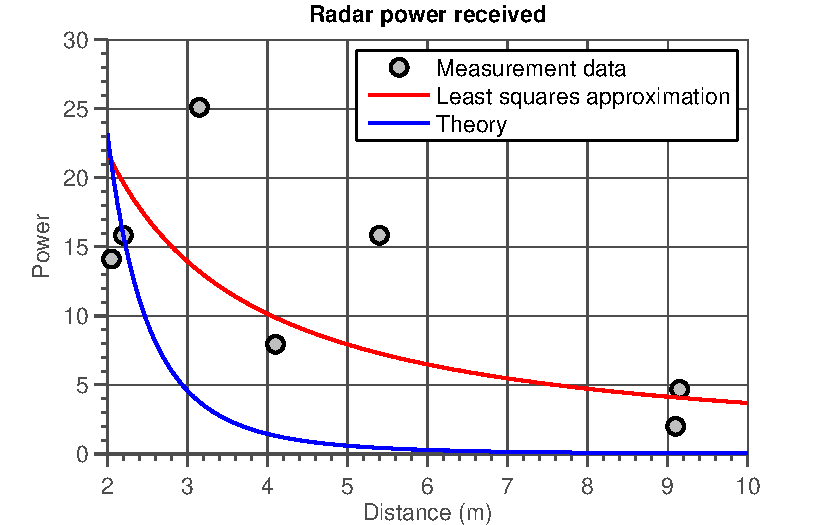
\includegraphics[width=.8\linewidth]{resource/fit.pdf}
	\end{center}
	\caption{Measurement of the power received by the radar}
	\label{fig:ass-2-power}
\end{figure}

Figure~\ref{fig:ass-2-power} shows the results. Theory states that the exponent of Equation~\ref{eq:ass-2-exp} should be $-4$. The deviation from this theoretical value can be explained using the geometry of the measurement arrangement. Waves reflect on the walls and doors of the narrow hallway. These reflections are a source of noise, which adds up to the power measured. Therefore, the total power measured is higher than the power caused by reflections on the measurement object. As the measurment object is placed further away from the radar, the noise increases. As a consequence, the power caused by reflections on the measurement object seems higher than its actual value.

Let us denote the power received at a distance $D$ by $P$. If we assume that $\operatorname{E}[P|D=x]=P(x)$, then, using a maximum-likelihood estimation, the standard deviation $\sigma$ is given by \num{15.8}, which is, considering the scale of the y-axis of Figure~\ref{fig:ass-2-power}, pretty bad.


\end{document}